\documentclass[a4paper,twoside,kulak]{kulakreport} %options: kul or kulak (default)

\usepackage[utf8]{inputenc}
\usepackage[dutch]{babel}
\usepackage{eurosym}
\usepackage[utf8]{inputenc}
\usepackage[dutch]{babel}
\usepackage{siunitx}
\usepackage{graphicx}
\usepackage{flafter}
\usepackage{pdfpages}
\usepackage{caption}
\usepackage{subcaption}
\usepackage{booktabs}
\usepackage{url}
\usepackage{hyperref}
\usepackage{gensymb}
\usepackage{tabularx,pbox}




\faculty{Wetenschap \& Technologie Kulak}
\group{Ingenieurswetenschappen}
\title{De \textit{automated microplate dispenser}}
\subtitle{Een zoektocht naar balans tussen precisie, snelheid en betaalbaarheid}
\author{Team ELISA}
\institute{Matthias Derez, Maxime Dujardin, Korneel Verkens, Seppe Vilain}
\date{Academiejaar 2019 -- 2020}
\address{
   KU Leuven Kulak           \\
   Wetenschap \& Technologie \\
   Etienne Sabbelaan 53, 8500 Kortrijk                \\
   
   }

\begin{document} % hier begint de eigenlijke inhoud van het document

\titlepage

\tableofcontents

\chapter*{Inleiding}
Vandaag de dag komen veel mensen in contact met HIV, de ziekte van Lyme en voedselallergenen. Een vaak gebruikte techniek om deze aandoeningen op te sporen, is de ELISA-test\cite{wikipedia} (\textit{Enzyme-Linked ImmunoSorbent Assay}). Het is een laboratoriumtest die gebruikt wordt voor het meten van macromoleculaire stoffen. Door, gebruik makend van een enzym als merker, een specifieke antigeen-antistofbinding aan te tonen in het bloed of andere lichaamsvloeistof van een mens of dier, kan de eventuele aanwezigheid van de aandoening vastgesteld worden. De ELISA-test heeft naast het opsporen van virussen en voedselallergenen nog tal van andere toepassingen\cite{ELISAApplications}. Zo kan men de test gebruiken om vroege fasen van eierstok- en borstkanker op te sporen, om concentraties illegale drugs te bepalen in urinestalen en om de concentratie van een medicijn in patiënten die een behandeling ondergaan, te monitoren. Nog een andere toepassing is het detecteren van humaan choriongonadotrofine, een hormoon dat tijdens de zwangerschap door de placenta wordt geproduceerd\cite{HumanChorionicGonadotropin}. \newline
Er bestaan verschillende varianten van de test. De meest eenvoudige versie is de directe antistof ELISA-test. Deze verloopt in volgende stappen (zie Figuur \ref{fig: directe ELISA}) \cite{AfbeeldingdirectELISA}:

\begin{figure}[h]
	\centering
	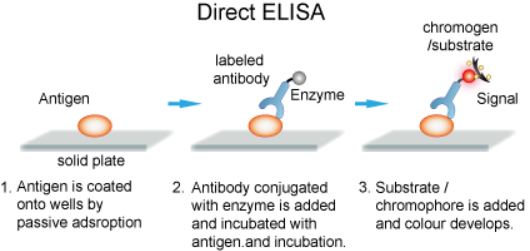
\includegraphics[width=0.5\textwidth]{ELISA.png}
	\caption{Directe antistof ELISA-test}
	\label{fig: directe ELISA}
	
\end{figure} 


\begin{figure}[h]
	\centering
	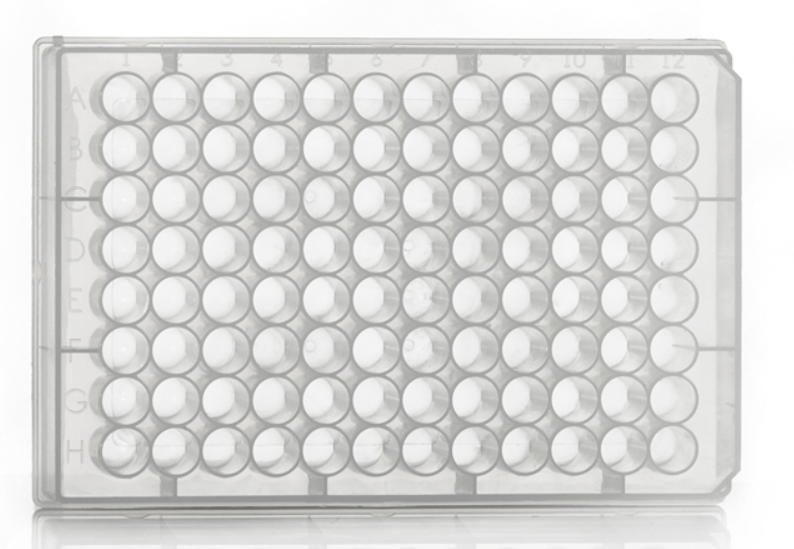
\includegraphics[width=0.5\textwidth]{microplate.png}
	\caption{Microwellplaat}
	\label{fig: microwellplaat}
	
\end{figure} 



\begin{enumerate}
	\item Men brengt het te bestuderen antigen aan in de \textit{wells} van een \textit{microwell}plaat (zie Figuur \ref{fig: microwellplaat}).
	\item Vervolgens wordt een oplossing met een niet-reagerend proteïne toegevoegd aan de wells zodat het volledige grondvlak van elke well bedekt is met vloeistof.
	\item Het antilichaam met een geconjugeerd enzyme wordt in de wells gevoegd.
	\item Een substraat voor het enzyme wordt toegevoegd. 
	\item De concentratie van het antilichaam wordt gemeten.
\end{enumerate}
Andere varianten zijn de indirecte \textit{sandwich} ELISA-, de competitieve inhibitie ELISA- en de \textit{blocking} ELISA-test\cite{soortenELISA}.
Deze test wordt elke dag gebruikt door de onderzoekers van het \textit{Laboratory for Thrombosis Research} aan KU Leuven Campus Kulak Kortrijk. Er is echter een probleem bij de uitvoering van de test: wanneer de uitvoering van het proces niet geautomatiseerd is, neemt de ELISA-test veel handenarbeid en tijd in beslag. De \textit{automated microplate dispenser} kan hier een oplossing voor bieden. Deze machine is volledig geautomatiseerd en snel, waardoor een pak efficiënter kan gewerkt worden. 

Het grote probleem met de \textit{automated microplate dispensers} die momenteel op de markt zijn (zie Figuur \ref{fig: microplateDispensers}), is dat prijzen de pan uit swingen. Voor een nieuw toestel betaalt men gemakkelijk \euro $12000$ tot \euro $35000$\cite{BioSPX} exclusief BTW, voor een tweedehandstoestel \euro 1500 tot \euro 8500\cite{LabX}. Het doel van dit project is dan ook om een machine te bouwen die dezelfde taken kan uitvoeren als de apparaten die momenteel op de markt zijn, maar dan voor een wél acceptabele prijs.

\begin{figure}
	\centering
	\begin{subfigure}{.5\textwidth}
		\centering
		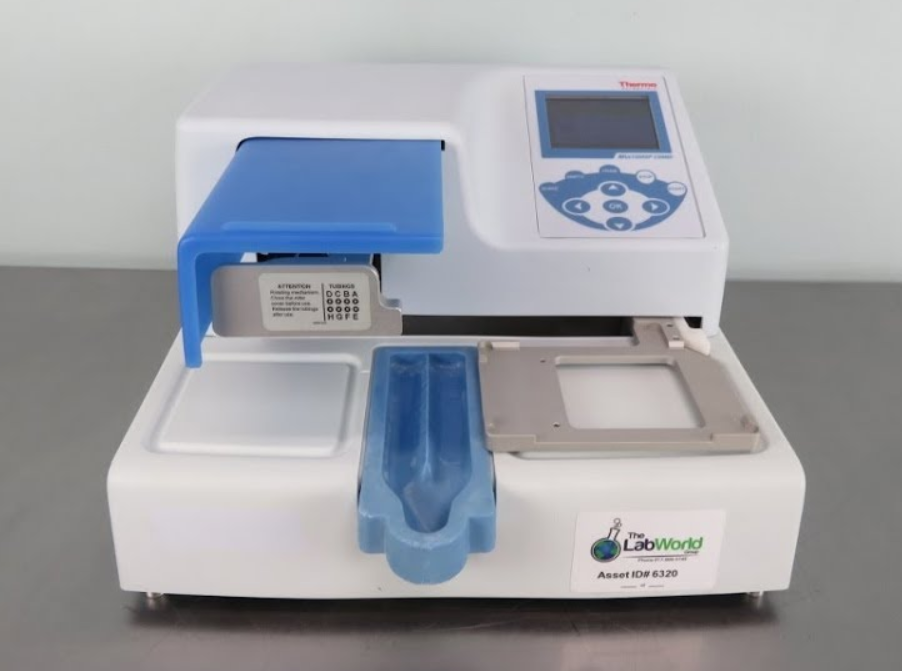
\includegraphics[width=0.9\linewidth]{microplateDispenserThermo.png}
	\end{subfigure}%
	\begin{subfigure}{.5\textwidth}
		\centering
		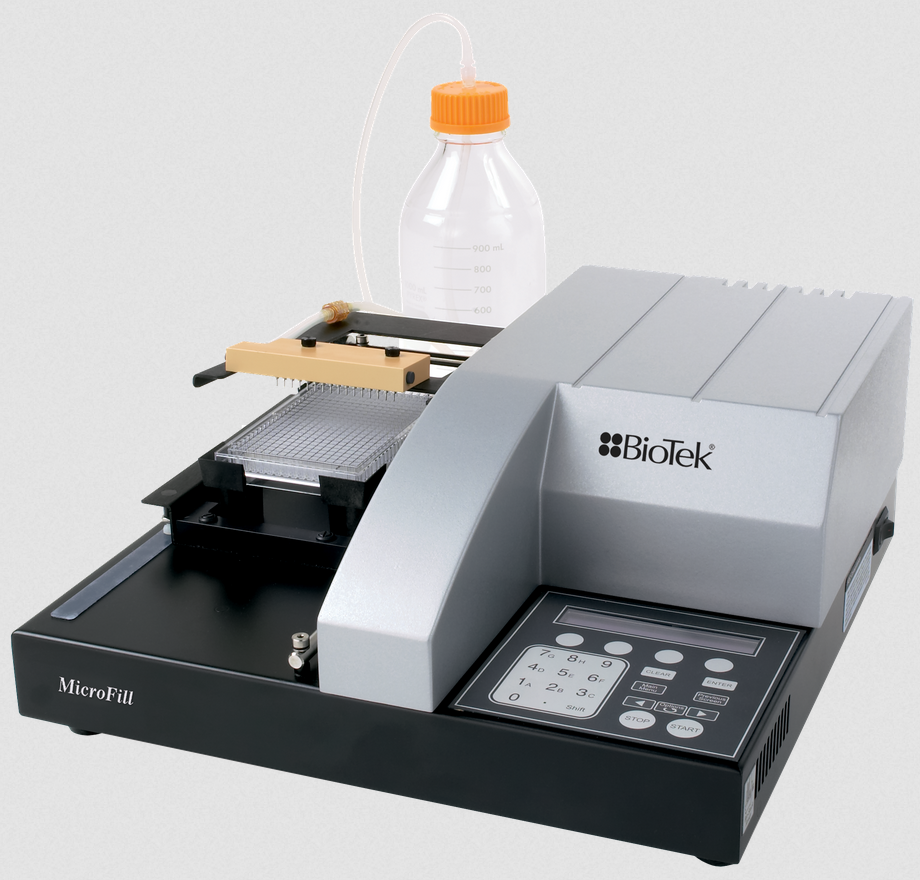
\includegraphics[width=0.9\linewidth]{microplateDispenserBioTek.png}
	\end{subfigure}
	\caption{Voorbeelden van automated microplate dispensers die op de markt zijn}
	\label{fig: microplateDispensers}
\end{figure}



\chapter{Klantenvereisten}
Het laboratorium voor trombose onderzoek wil een geautomatiseerde \textit{dispenser}. De \textit{dispenser} moet in staat zijn om volledig autonoom een \textit{microwell}-plaat te vullen met de te onderzoeken substantie. Dit proces moet foutloos gebeuren: in elke \textit{microwell} moet exact evenveel substantie zitten en er mag er uiteraard niet naast de \textit{microwells} gespoten worden. Bovendien moet dit alles kunnen in een tijd die aanzienlijk korter is dan wanneer men deze \textit{microwell}-plaat handmatig zou vullen. Vooral dit laatste aspect is belangrijk, aangezien het handmatig vullen van de platen een zeer arbeidsintensief en tijdrovend onderdeel is van de ELISA-test. Het apparaat moet eenvoudig te bedienen zijn en de pipetpunten die de substantie in de wells spuiten, moeten vervangbaar zijn.  Indien mogelijk kunnen ook al andere stappen, buiten het vullen van de \textit{microwells} zelf, geautomatiseerd worden. Het automatisch aan- en afvoeren van microwellplaten kan het productieproces al veel versnellen. Er is een budget van \euro 50 tot \euro 75 voorzien.
\chapter{Ontwerpspecificaties}
De te onderzoeken substantie bevindt zich in een recipiënt van waaruit het kan worden opgezogen. De \textit{microwell}-plaat is \SI{127.76}{mm} breed, \SI{85.48}{mm} lang en \SI{14.4}{mm} hoog. Er zitten 96 \textit{microwells} in, met een bovendiameter van \SI{6.96}{mm} en een benedendiameter van \SI{6.58}{mm} (zie Figuur \ref{fig: afmetingenMicrowellplaat}). Het werkvolume van elke well is tussen 25 $\mu l$ en 340 $\mu l$. De middelpunten van de wells bevinden zich op \SI{9}{mm} van elkaar. De middelpunten van de pipetpunten moeten dus op een afstand van \SI{9}{mm} van elkaar liggen en moeten verwijderbaar zijn. De machine moet elke well kunnen vullen met een hoeveelheid van 100 $\mu l$ of 200 $\mu l$ van de te onderzoeken substantie. Om de vloeistof niet te morsen naast de wells, moeten de pipetpunten telkens exact boven het middelpunt van de well de vloeistof lossen. Om het apparaat gebruiksvriendelijk te maken, moet een grafische interface voorzien worden. Zo kan de machine in enkele tellen opgestart worden en kunnen onderzoekers die de programmeertaal niet kennen de machine toch zonder probleem gebruiken.

\begin{figure}[h]
	\centering
	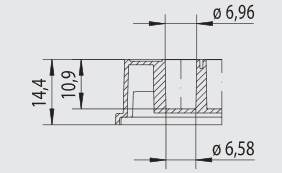
\includegraphics[width=0.5\textwidth]{AfmetingenMicrowell.png}
	\caption{Afmetingen \textit{microwell}}
	\label{fig: afmetingenMicrowellplaat}
	
\end{figure} 


\chapter{\textit{Concept}} 


In dit hoofdstuk wordt het uiteindelijke concept toegelicht en uitgelegd waarom dit concept weerhouden is.

\section{Werking}

	Het concept (zie Figuren \ref{fig: CAD-model bovenaan} en \ref{fig: CAD-model onderaan}) laat toe om zes microwell-platen met één druk op de startknop te vullen. Er wordt gewerkt met twee pompen die de vloeistof oppompen uit het recipiënt waarin de te onderzoeken substantie zich bevindt. Op elke pomp is een buizennetwerk aangesloten. In elk buizennetwerk wordt de vloeistof verdeeld over uiteindelijk acht pipetpunten. De middelpunten van de pipetpunten bevinden zich telkens op een afstand van \SI{9}{mm} van elkaar. De verdeling gebeurt door elke buis te splitsen in twee nieuwe buizen m.b.v. een T-verdeelstuk. De pipetpunten kunnen van de machine gehaald worden en zo gemakkelijk vervangen worden.
	
	Alle onderdelen van de constructie zijn bevestigd aan het centrale chassis. Dit vormt de basis van de gehele constructie en bestaat uit 4 profielen die aan elkaar vasthangen. Het hierboven beschreven buizennetwerk wordt hierop vastgemaakt.
	De microplates worden op een transportplaat geplaatst. Op dit platform is plaats voorzien voor 6 microplates: deze worden in 2 rijen van 3 na elkaar gezet. Het platform is vastgemaakt aan een aandrijfriem, die op zijn beurt verbonden is met een motor. De transportplaat wordt m.b.v. lagers verbonden aan 2 staven en kan zo vrij heen en weer bewegen. De staven zijn gemonteerd op het chassis.
	
	Het mechanisme om de microwells te vullen werkt als volgt: telkens wanneer een rij van acht wells gevuld is, stopt de pomp en verschuift de transportplaat. Daarna vult de pomp opnieuw acht wells. Dit proces wordt herhaald tot de twaalf rijen van acht wells gevuld zijn. 
	
\section{Voordelen ontwerp}
	We gebruiken slechts 8 pipetpunten en geen 12 of 96. Er werd beslist om geen 96 wells tegelijk te vullen omdat één enkele pomp niet genoeg zuigkracht genereert om zo'n grote hoeveelheid vloeistof te kunnen opzuigen. De reden dat we geen 12 wells tegelijk vullen is de volgende: wanneer we de vloeistof verdelen over 8 pipetpunten, kunnen we ervoor zorgen dat de vloeistof van het recipiënt tot aan elk van de 8 pipetpunten een gelijke afstand aflegt. Dit kan eenvoudig gerealiseerd worden door de buizen te splitsen m.b.v. T- of Y-verdeelstukken, wat bij 12 pipetpunten niet het geval is. Dit laatste zou ervoor kunnen zorgen dat er niet evenveel vloeistof in elke well komt, wat problemen oplevert bij het uitvoeren van de ELISA-test. Dit concept heeft ook als voordeel t.o.v. andere mogelijke concepten dat er maar één bewegend onderdeel is. Hierdoor kan het aantal motoren beperkt worden. Een ander voordeel is dat het relatief goedkoop is. Bij andere concepten die gemaakt werden, werd voorgesteld om met cilinders en zuigers te werken in plaats van met een pomp. Deze onderdelen kosten per stuk echter even veel als het voorziene budget voor dit project. Door met een pomp te werken kan dit vermeden worden en wordt de kostprijs aanzienlijk gedrukt. 
	
\begin{figure}[h]
	\centering
	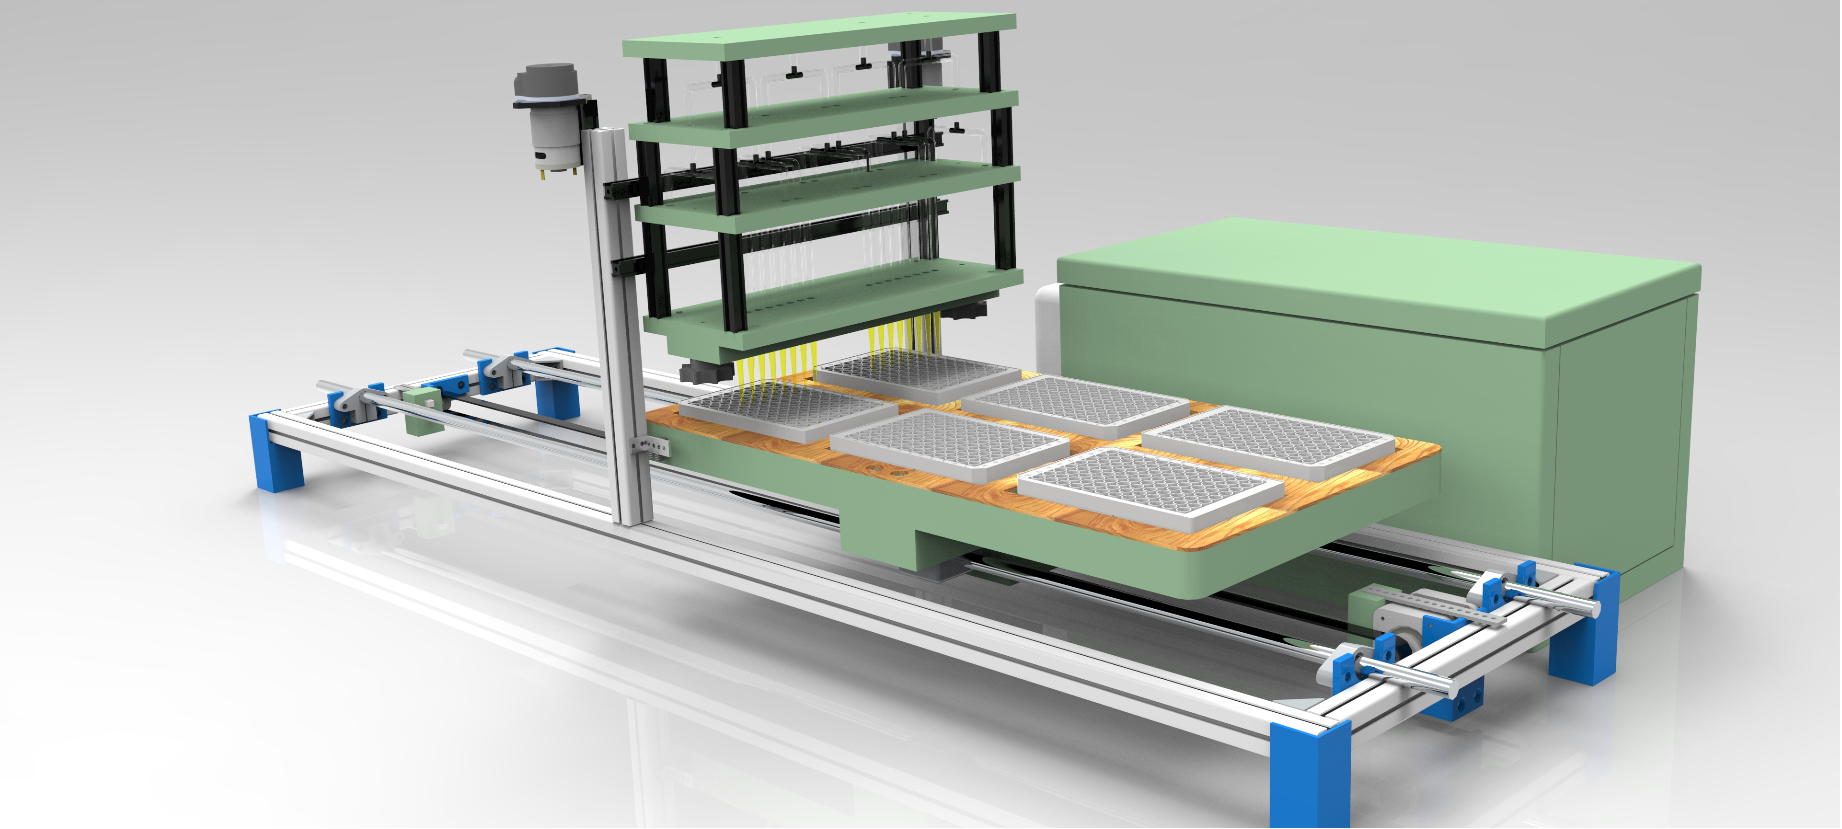
\includegraphics[width=\textwidth]{renderingBovenaan.png}
	\caption{CAD-model van onze automated microplate dispenser}
	\label{fig: CAD-model bovenaan}
	
\end{figure} 

\begin{figure}[h]
	\centering
	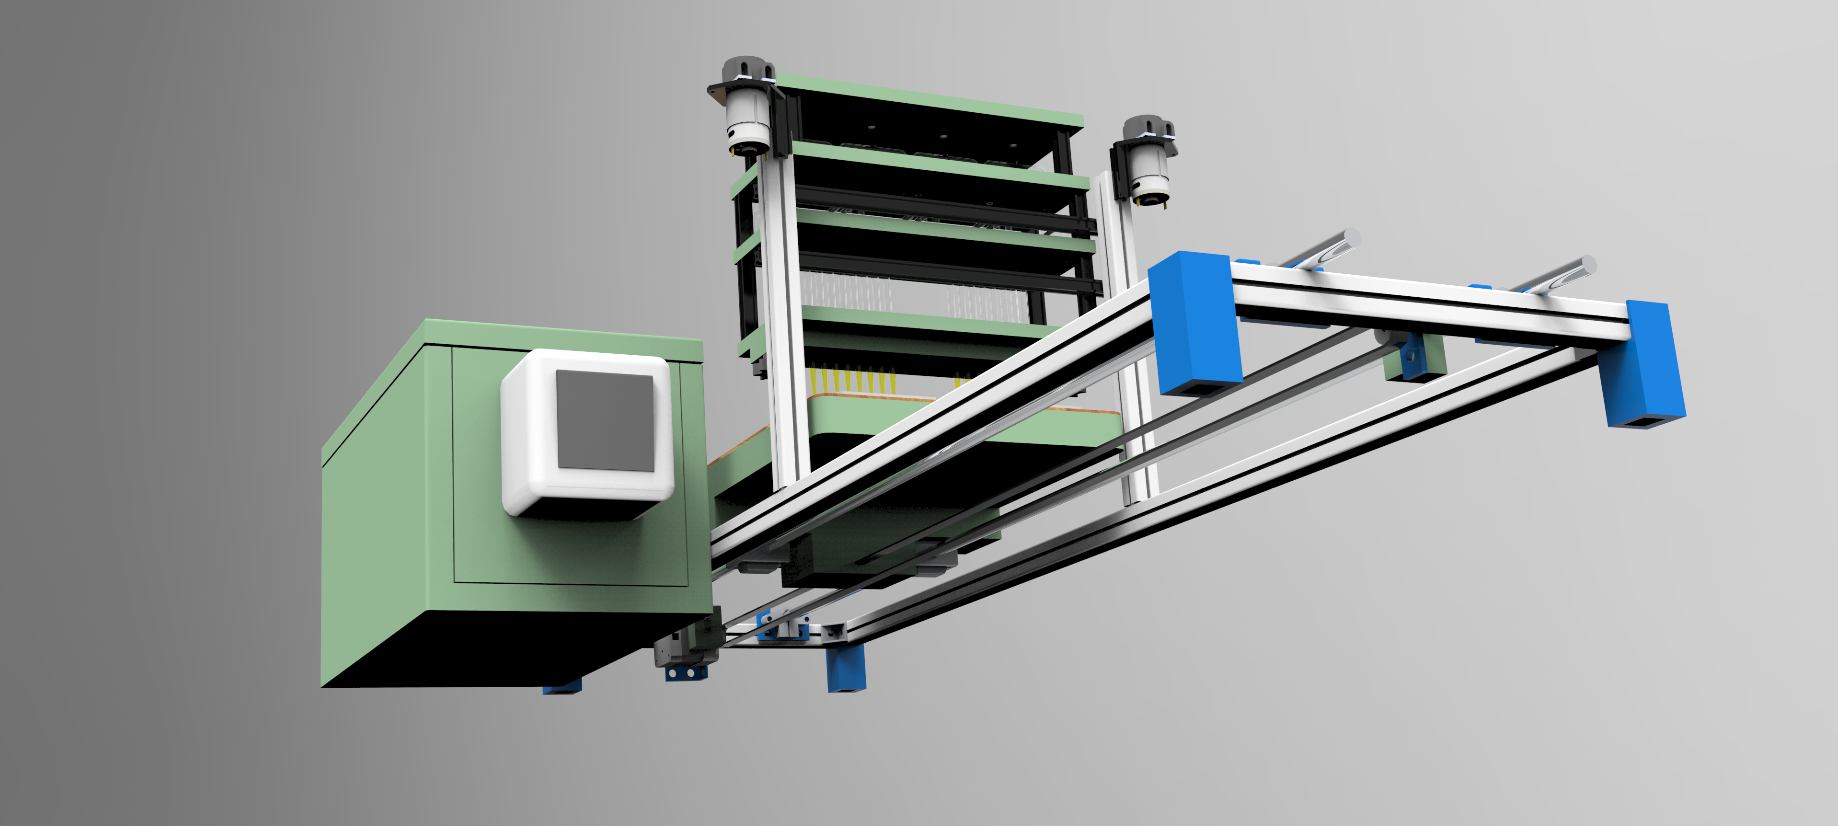
\includegraphics[width=0.8\textwidth]{renderingOnderaan.png}
	\caption{Onderaanzicht van onze automated microplate dispenser}
	\label{fig: CAD-model onderaan}
	
\end{figure} 


\chapter{Realisatie ontwerp}

In dit hoofdstuk wordt uitgelegd hoe we het ontwerp dat in het vorige hoofdstuk toegelicht werd, gerealiseerd hebben. We bespreken de belangrijkste onderdelen die we gebruikt hebben en leggen uit waarom precies voor deze onderdelen werd gekozen. Een overzicht van de aangekochte onderdelen is terug te vinden in het financieel verslag (zie appendix \ref{Appendix: Financieel verslag}).

\section{Chassis}

Het chassis dient als basis voor het hele toestel. De belangrijkste vereisten voor dit onderdeel is dat het stevig en licht moet zijn. Om hieraan te voldoen, beslisten we om het chassis op te bouwen uit 4 aluminium profielen die aan elkaar bevestigd werden. 

\section{Transportplaat}

De transportplaat waarop de microplates worden geplaatst, laat toe om 6 microplates tegelijk te vullen. Om te voorkomen dat er vloeistof naast de wells gespoten wordt, is het noodzakelijk dat de microplates niet kunnen verschuiven tijdens het verplaatsen van de transportplaat. Om dit schuiven te vermijden, werden uit een dunne houten plaat (met dezelfde afmetingen als de transportplaat) 6 rechthoeken \textit{gelasercut} met precies de afmetingen van een microplate. Dit geheel werd bevestigd op de transportplaat. Als materiaal voor de transportplaat kozen we voor waterafstotend MDF (\textit{Medium-Density Fibreboard}). Dit materiaal heeft twee voordelen. Ten eerste is het een licht materiaal, wat een relatief lage belasting voor de constructie betekent. Een tweede voordeel is dat de transportplaat niet zal vergaan als er vloeistof op de plaat terechtkomt, wat bij een gewone houten plaat wel het geval zou zijn.  \\


AFBEELDING TRANSPORTPLAAT ZETTEN



\section{Steppermotor}

Als motor werd gekozen voor een \textit{steppermotor}. Een steppermotor is een type motor dat werkt m.b.v. elektromagneten die de aandrijfas van de motor laten draaien. In de door ons gebruikte motor zitten in totaal 4 elektromagneten die afwisselend aan- en uitgezet worden door er een stroom door te sturen. Telkens 1 van de 4 magneten wordt aangezet (dit is 1 stap), verdraait de aandrijfas waarop het magnetisch veld van de aangezette elektromagneet inwerkt volgens een vaste hoek\footnote{Voor meer informatie i.v.m. steppermotoren verwijzen we naar \url{https://en.wikipedia.org/wiki/Stepper_motor}}. Het grote voordeel van dit type motoren is dat deze hoek zeer klein is: de as van de motor die wij gebruiken maakt per stap een verdraaiing van $1.8\degree$. Hierdoor kunnen we de transportplaat die via een aandrijfriem aan de motor verbonden is met een zeer hoge nauwkeurigheid verplaatsen. Dit is van groot belang gezien de kleine afstand tussen twee opeenvolgende rijen wells op de microplates. 

\section{Waterpomp}

De gebruikte pompen zijn vacuümpompen. Deze zorgen ervoor dat wanneer de pomp niet actief is dat de vloeistof die nog in het buizennetwerk zit niet weglekt via de pipetpunten. We kozen zoals eerder vermeld voor twee pompen die de twee buizennetwerken van vloeistof voorzien. 

\section{Microcontroller}

Om aan de vereiste te voldoen dat de machine volledig automatisch de microplates kan vullen, moet het apparaat bestuurd worden via een microcontroller. Er werd gekozen voor een \textit{Raspberry Pi}. Deze heeft verschillende voordelen t.o.v. andere microcontrollers. Ten eerste is het een relatief goedkope microcontroller. Dit was een belangrijk aspect gezien het budget dat voorhanden was. Ten tweede laat een Raspberry Pi toe om een HDMI-kabel en computermuis rechtstreeks aan te sluiten op de microcontroller. Dit laat toe om een grafische interface te implementeren die eenvoudigweg kan bediend worden via een scherm en computermuis die met de Raspberry Pi verbonden zijn. Een derde reden voor onze keuze is dat dit type microcontroller redelijk compact is in vergelijking met andere microcontrollers die te verkrijgen zijn. Tot slot werkt een Raspberry Pi met de programmeertaal \textit{Python}. Dit had voor ons als voordeel dat we al konden werken met deze taal, wat niet het geval was met bijvoorbeeld een \textit{Arduino}microcontroller. 



\chapter{Programmeerstructuur}

In dit hoofdstuk wordt uitgelegd hoe de programma's die de machine besturen opgebouwd zijn.

\section{Grafische interface}
Wanneer men de stekker van het toestel in het stopcontact plaatst en de schakelaar op 'Aan' zet, zal het scherm vanzelf opstarten en verschijnt de grafische interface (zie Figuur \ref{fig: Grafische interface}). In de grafische interface kan de gebruiker selecteren welke actie de machine moet uitvoeren. De mogelijkheden zijn: \textit{initialize}, \textit{cleanup}, \textit{quit} en een of meerdere microplates vullen (zie figuur \ref{fig: Grafische interface}). Deze interface is in de programmeertaal \textit{Python} geprogrammeerd. 

\begin{figure}
	\centering
	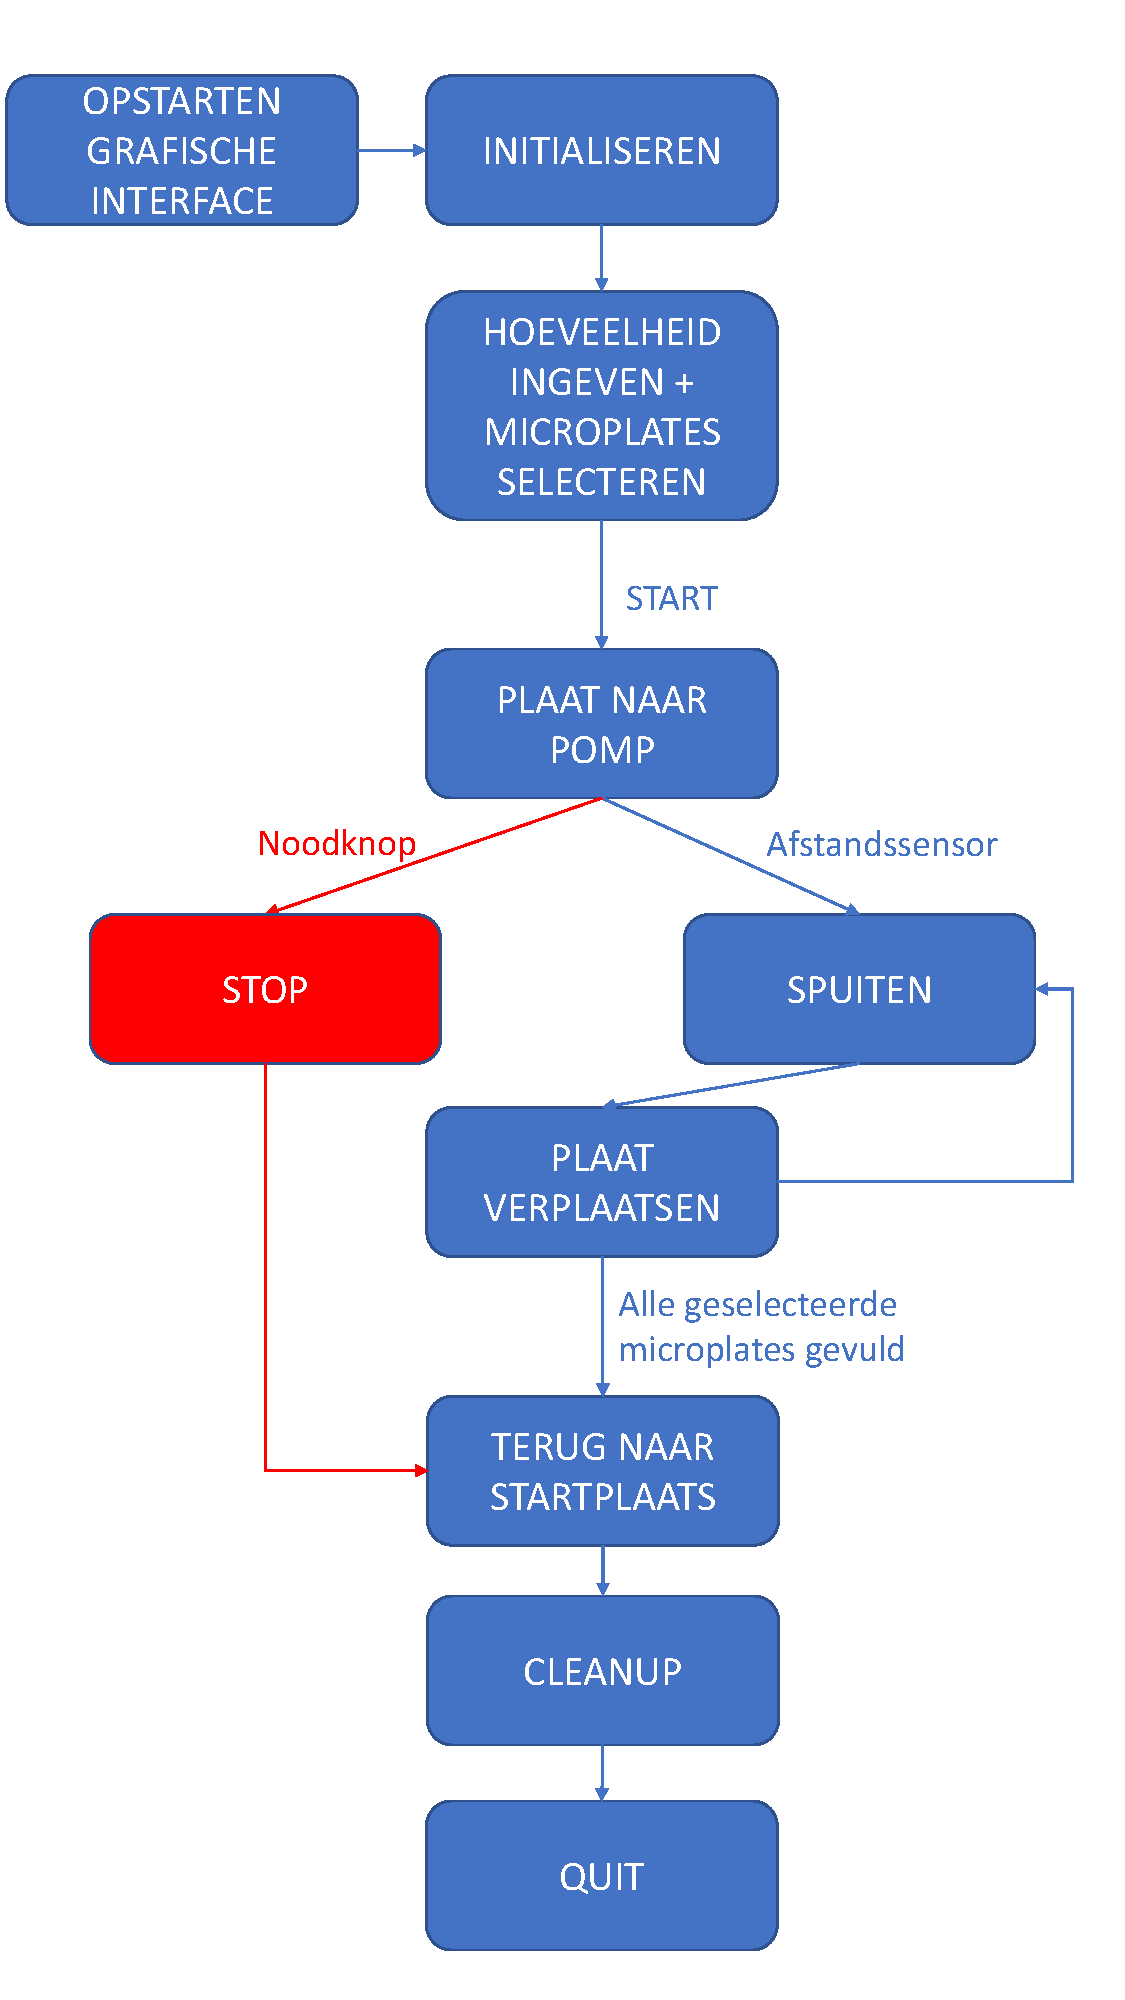
\includegraphics[width=1\textwidth]{Programmastructuur.pdf}
	\caption{Programmastructuur}
	\label{fig: Programmastrucuur}
	
\end{figure} 

\section{Programmastructuur}
Om de machine zo autonoom mogelijk te laten werken, volgen we volgende programmastructuur (zie Figuur \ref{fig: Programmastrucuur}). 

\paragraph{Initialize} 

Eens de Raspberry Pi is opgestart, ziet men de grafische interface op het scherm. Alvorens de microplates gevuld kunnen worden, moeten de leidingen van het apparaat gevuld worden met de nodige substantie. Hiervoor kan men de knop 'INITIALIZE' selecteren (zie 'B' in Figuur \ref{fig: Grafische interface}). Men kan kiezen om maar één van de twee pompen of om beide te initialiseren (zie 'C' in Figuur \ref{fig: Grafische interface}). 
\paragraph{Hoeveelheid ingeven + microplates selecteren}
Na het initialiseren, selecteert men de gewenste hoeveelheid vloeistof die in elke microwell moet komen (zie 'F' in Figuur \ref{fig: Grafische interface}) en welke microplates gevuld moeten worden (zie 'G' en 'H' in Figuur \ref{fig: Grafische interface}). Door de startknop (zie 'I' in Figuur \ref{fig: Grafische interface}) te selecteren, begint de machine met het uitvoeren van de gevraagde taken. 
\paragraph{Plaat naar pomp}
De transportplaat beweegt vooruit, in de richting van de pipetpunten, tot een afstandssensor de plaat 'ziet' en een signaal doorgeeft aan de microcontroller. Daarna is er een afwisselend proces van een kleine hoeveelheid vloeistof die in de wells wordt gepompt en een kleine verplaatsing van de transportplaat. Zo worden de rijen met wells van de microplate één voor één gevuld. Dit gaat door tot de wells van alle microplates gevuld zijn.
\paragraph{Noodstop}
Wanneer de afstandssensor echter geen signaal doorgeeft, zou de transportplaat rechtdoor blijven  bewegen. Zo zou er schade kunnen ontstaan wanneer de plaat het einde van het chassis bereikt. Om dit te voorkomen is er een noodknop bevestigd aan de andere kant van het chassis. Wanneer deze wordt ingedrukt, stopt de transportplaat onmiddellijk met vooruitgaan en begeeft deze zich terug naar  zijn startpositie. 
\paragraph{Terug naar startplaats}
In beide gevallen, wanneer alle wells gevuld zijn of de noodknop ingedrukt wordt, begeeft de transportplaat zich uiteindelijk terug naar zijn startpositie. Hiervoor is er een andere drukknop bevestigd aan het chassis. Zo kan de transportplaat achteruit blijven bewegen, totdat deze drukknop wordt ingedrukt en de transportplaats dus terug op zijn startpositie staat. 

\paragraph{Cleanup}
Wanneer men klaar is met het vullen van microplates, moet men de leidingen ledigen. Hiervoor kan men de functie 'CLEANUP' gebruiken (zie 'A' in Figuur \ref{fig: Grafische interface}).
\paragraph{Quit}
Om de microcontroller correct af te sluiten en zo schade te voorkomen, dient men de functie 'QUIT' te gebruiken (zie 'E' in Figuur \ref{fig: Grafische interface})

\begin{figure}[h]

	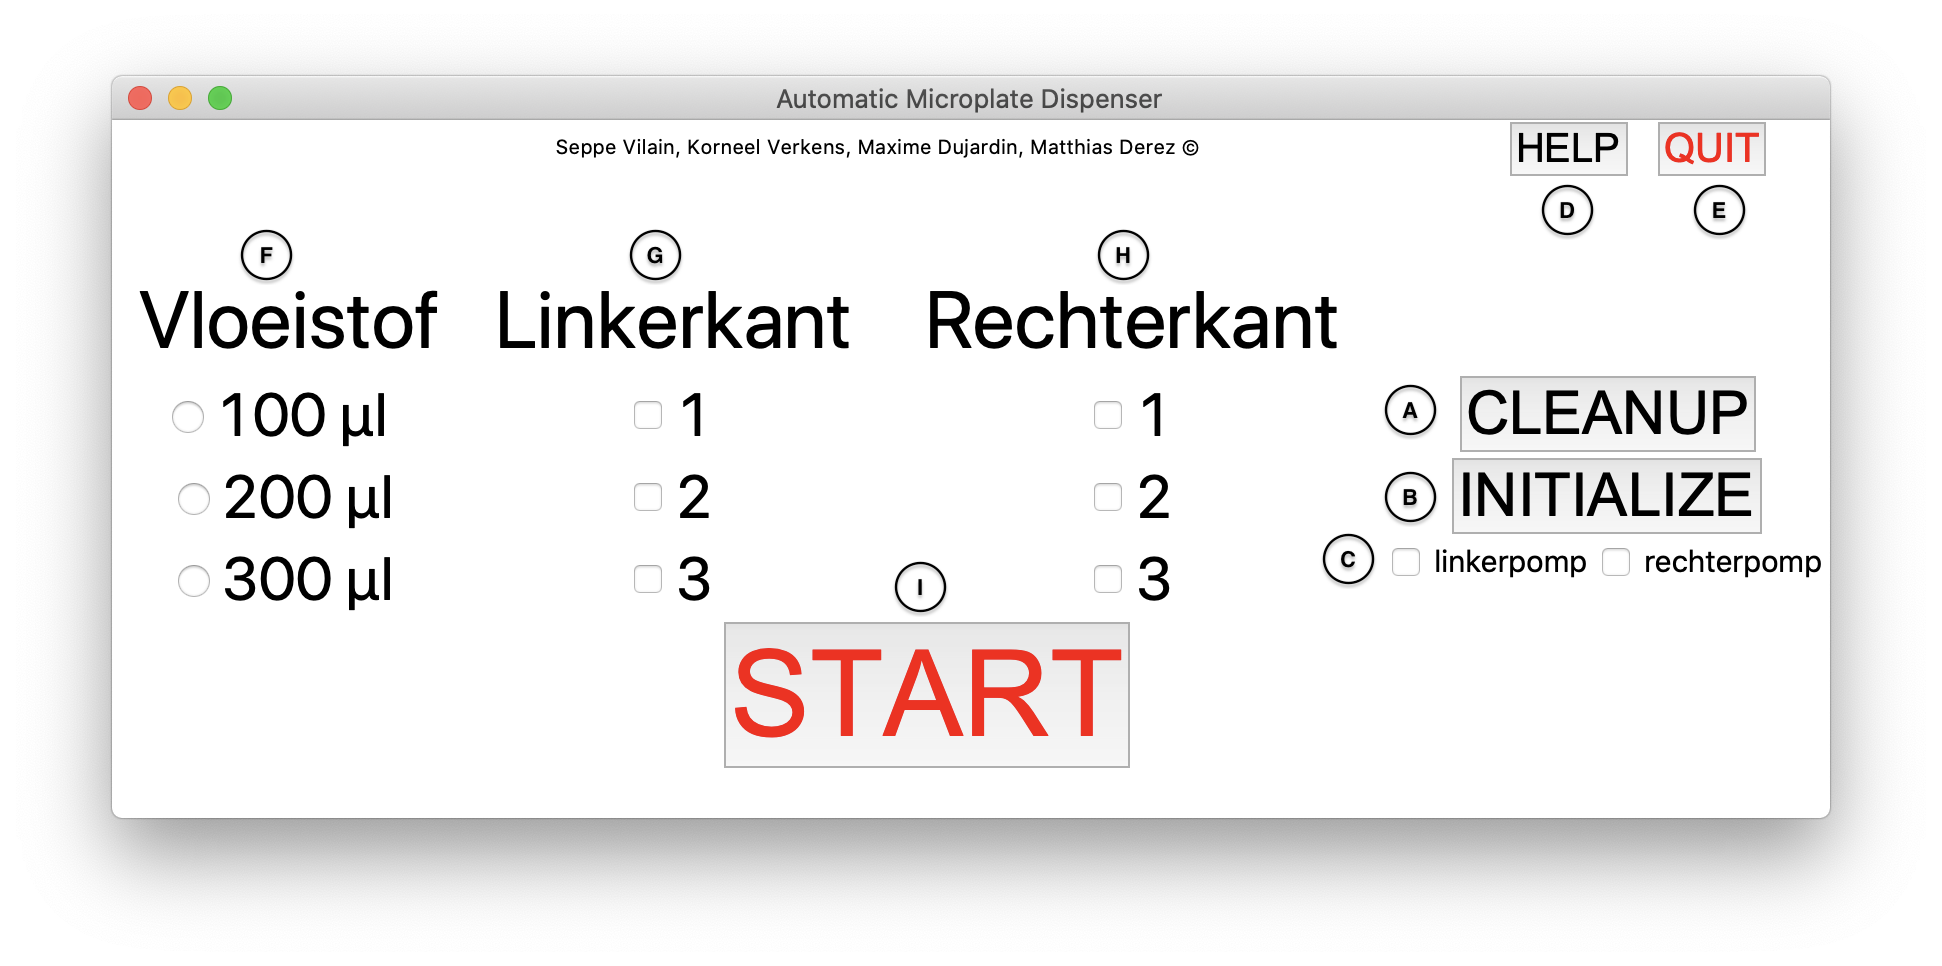
\includegraphics[width=1.3\linewidth]{GI_letters.png}
	\caption{Grafische Interface}
	\label{fig: Grafische interface}
	
\end{figure} 



\chapter{\textit{Unique selling proposition}}

De gebouwde machine heeft heel wat potentieel. Hieronder vindt u enkele grote pluspunten die onze machine onderscheidt van toestellen die reeds op de markt zijn.

\paragraph{Prijs-kwaliteitverhouding}

Het grootste voordeel van ons toestel t.o.v. andere toestellen is ongetwijfeld de uitstekende prijs-kwaliteitverhouding. Ons toestel kost in totaal \euro 173.63 (dit is weliswaar zonder werkuren te verrekenen), wat 60 tot 200 keer minder is dan de prijs van andere toestellen. De machine werkt minder precies dan professionele toestellen, maar desalniettemin is de prijs-kwaliteitverhouding is uitstekend.

\paragraph{Gebruiksgemak}

Doordat alles geautomatiseerd is, hoeft de gebruiker van het apparaat zeer weinig te doen om de microwellplaten te vullen. Men hoeft enkel het aantal te vullen platen en het volume per microwell te specificeren en de microwellplaten op de transportband te plaatsen. Het ingeven van de aantallen en volumes kan heel snel en eenvoudig gebeuren via de voorziene grafische interface. De interface is zeer eenvoudig te bedienen via een scherm en computermuis. Er is een handleiding voorzien zodat de gebruiker snel aan de slag kan.

\paragraph{Mobiliteit en stevigheid}

Tijdens het ontwerp en materiaalkeuze werd zo veel mogelijk rekening gehouden met de massa van het toestel. De gehele machine is gebouwd op een chassis uit aluminium om een stevige basis te bekomen. Het platform op het chassis werd vervaardigd uit hout om zo veel mogelijk gewicht te besparen. Dit levert een licht, maar stevig geheel op. 

\paragraph{Vervangstukken}

De machine werd gemaakt uit onderdelen die gemakkelijk te verkrijgen zijn. Dit zorgt ervoor dat de gebruiker in het geval van een defect onderdeel snel kan geholpen worden en direct weer aan de slag kan.

\chapter{Mogelijkheden tot uitbreiding en verbetering}

Om nog beter aan de wensen van de klant te voldoen, zijn er nog enkele zaken die na het einde van dit project verbeterd kunnen worden. \\ \\
Ten eerste wordt de vloeistof niet precies genoeg over de microwells verdeeld om de ELISA-test op een wetenschappelijk verantwoorde manier uit te voeren. Om het apparaat te gebruiken om ook daadwerkelijk volledig zelf een ELISA-test uit te voeren, moet de verdeling van de vloeistof dus nog preciezer gebeuren. \\ \\
Ten tweede zou een optie kunnen voorzien worden die automatisch de pipetpunten vervangt indien dit de gebruiker dit wenst. \\ \\

Ten derde zou er een systeem kunnen voorzien worden dat automatisch een recipiënt onder de pipetpunten plaatst om de machine te initialiseren. Nu moet dit manueel gebeuren. Daarnaast zou ervoor gezorgd kunnen worden dat wanneer men de buizen ledigt, de vloeistof terug vloeit naar de recipiënt waar het vandaan komt. Zo moet er geen afzonderlijk recipiënt onder de pipetten gehouden worden. \\ \\

Een laatste mogelijke verbetering is een mechanisme dat automatisch gevulde microplates  van de transportplaat haalt en nieuwe microplates op de transportplaat plaatst. Nu moet de gebruiker van het apparaat dit zelf doen. Door ervoor te zorgen dat dit proces volledig geautomatiseerd wordt, kan het vullen van de microplates nog efficiënter gebeuren en moet de gebruiker minder zelf tussenkomen. \\ \\

%Daarnaast zou de dunne houten plaat die nu op de transportplaat ligt ook waterafstotend gemaakt kunnen worden. Deze bestaat nu uit normaal MDF en kan dus niet goed tegen water. De plaat vervangen door een dunne waterafstotende MDF-plaat of er een waterafstotende verf op spuiten zijn enkele van de mogelijke oplossingen. \\ \\


\chapter{Conclusie}

De automated microplate dispenser is een toestel dat het uitvoeren van de ELISA-test  efficiënter maakt. Deze machine kan snel en autonoom een te onderzoeken substantie verdelen over verschillende microwells. Een groot probleem met de toestellen die op de markt zijn, is dat ze zeer duur zijn. Met het door ons gebouwde toestel kan men veel sneller microplates vullen dan wanneer men deze handmatig zou pipetteren en dat voor een relatief lage prijs. Het grote probleem met onze machine is echter de precisie. Waar een professioneel, duur toestel tot op de microliter precies de substantie in de wells kan spuiten, is ons toestel niet nauwkeurig genoeg om de ELISA-test op een wetenschappelijk verantwoorde manier uit te voeren. Dit is niet geheel onlogisch, aangezien één van de redenen waarom deze toestellen zo duur zijn, net is omdat ze zo precies geijkt zijn. Met het budget en de tijd die wij ter beschikking hadden, konden we dit jammer genoeg niet realiseren. Ons toestel kan echter wel gebruikt worden om de microplates te wassen. Door alleen dit onderdeel van de ELISA-test al te automatiseren, kan in labo's heel wat tijd bespaard worden.

\clearpage
\nocite{wikipedia,LabX}
\bibliographystyle{unsrt}
\bibliography{bibliografie}

\chapter*{Appendices}

\section*{Handleiding toestel}

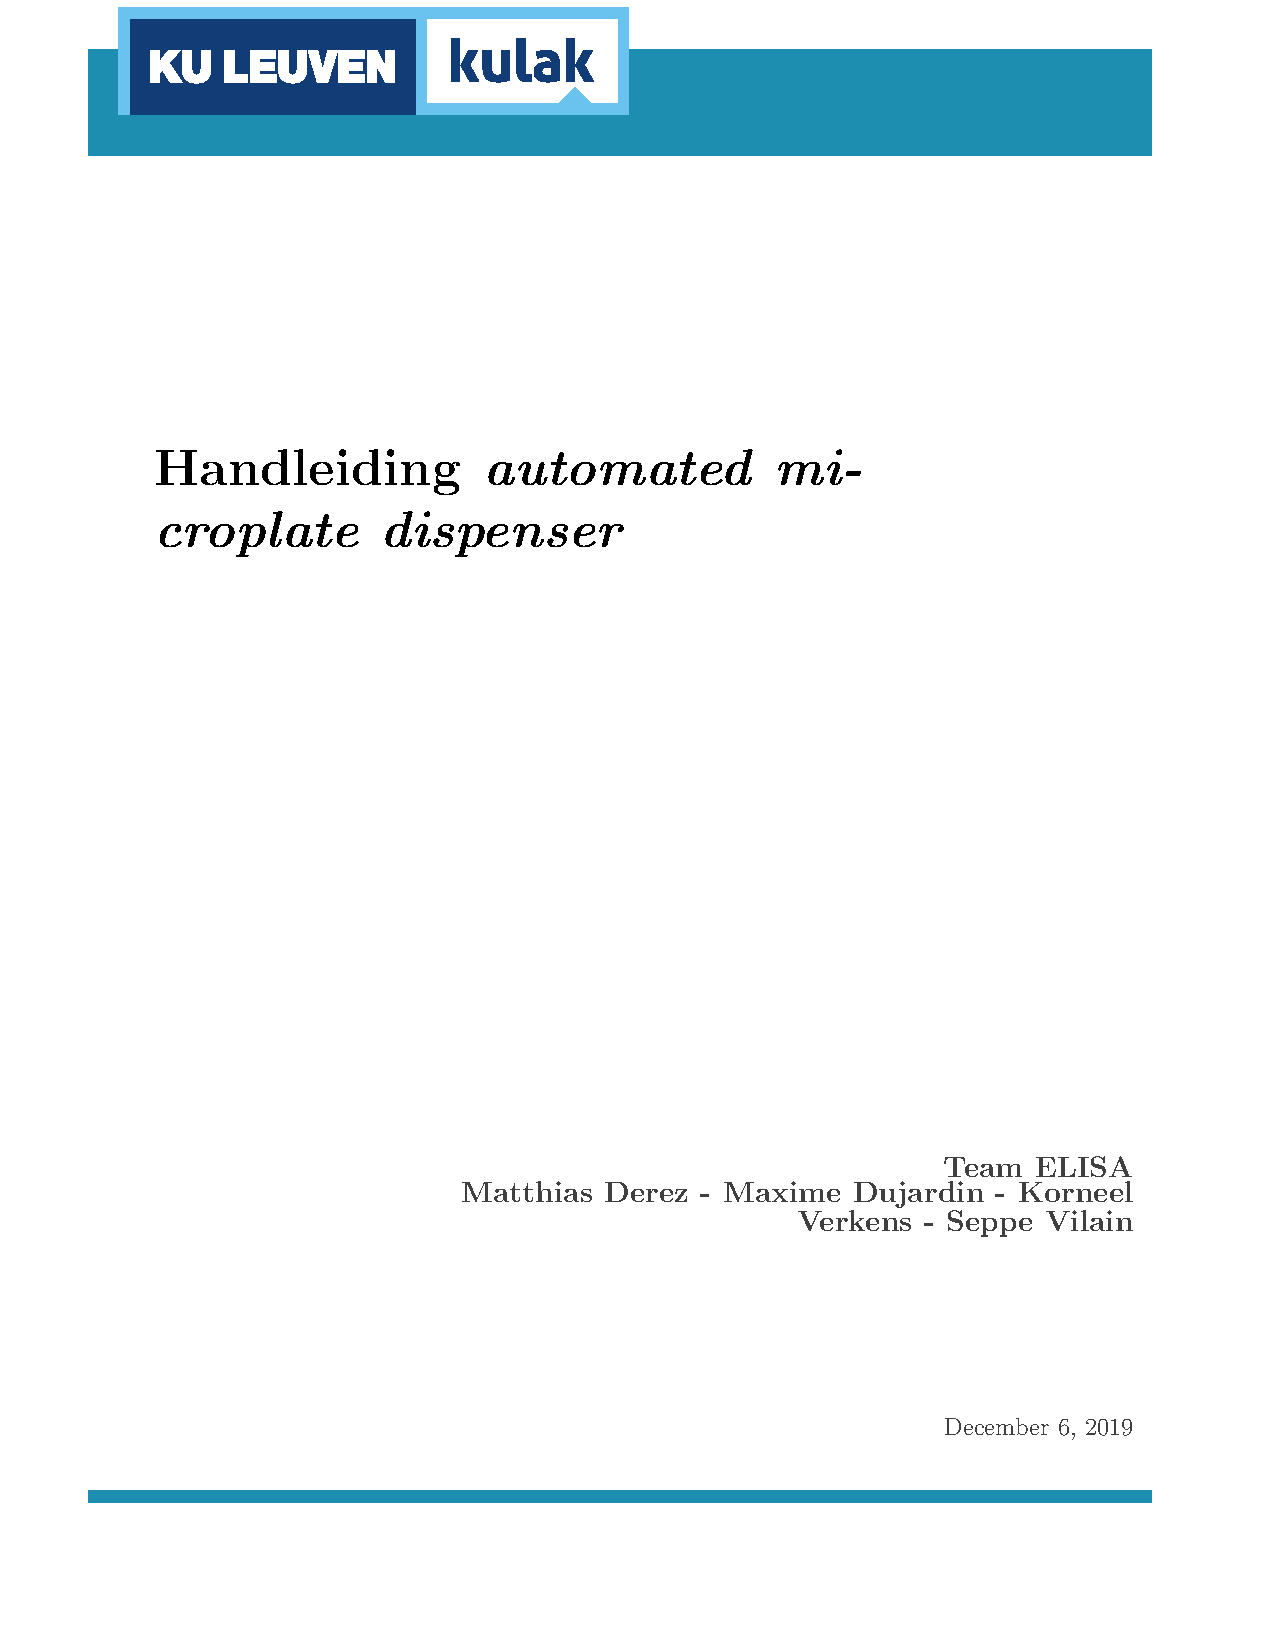
\includepdf[pages={1-}]{handleidingELISA.pdf}

\section*{Financieel verslag}
\label{Appendix: Financieel verslag}

In Tabel \ref{tab:financieelVerslag} staat een stuklijst met de gemaakte aankopen vermeld (de verschillende onderdelen vindt u in Figuren \ref{fig: renderingBovenkantStuklijst} en \ref{fig: renderingOnderkantStuklijst}). 


\begin{figure}[h]
	\centering
	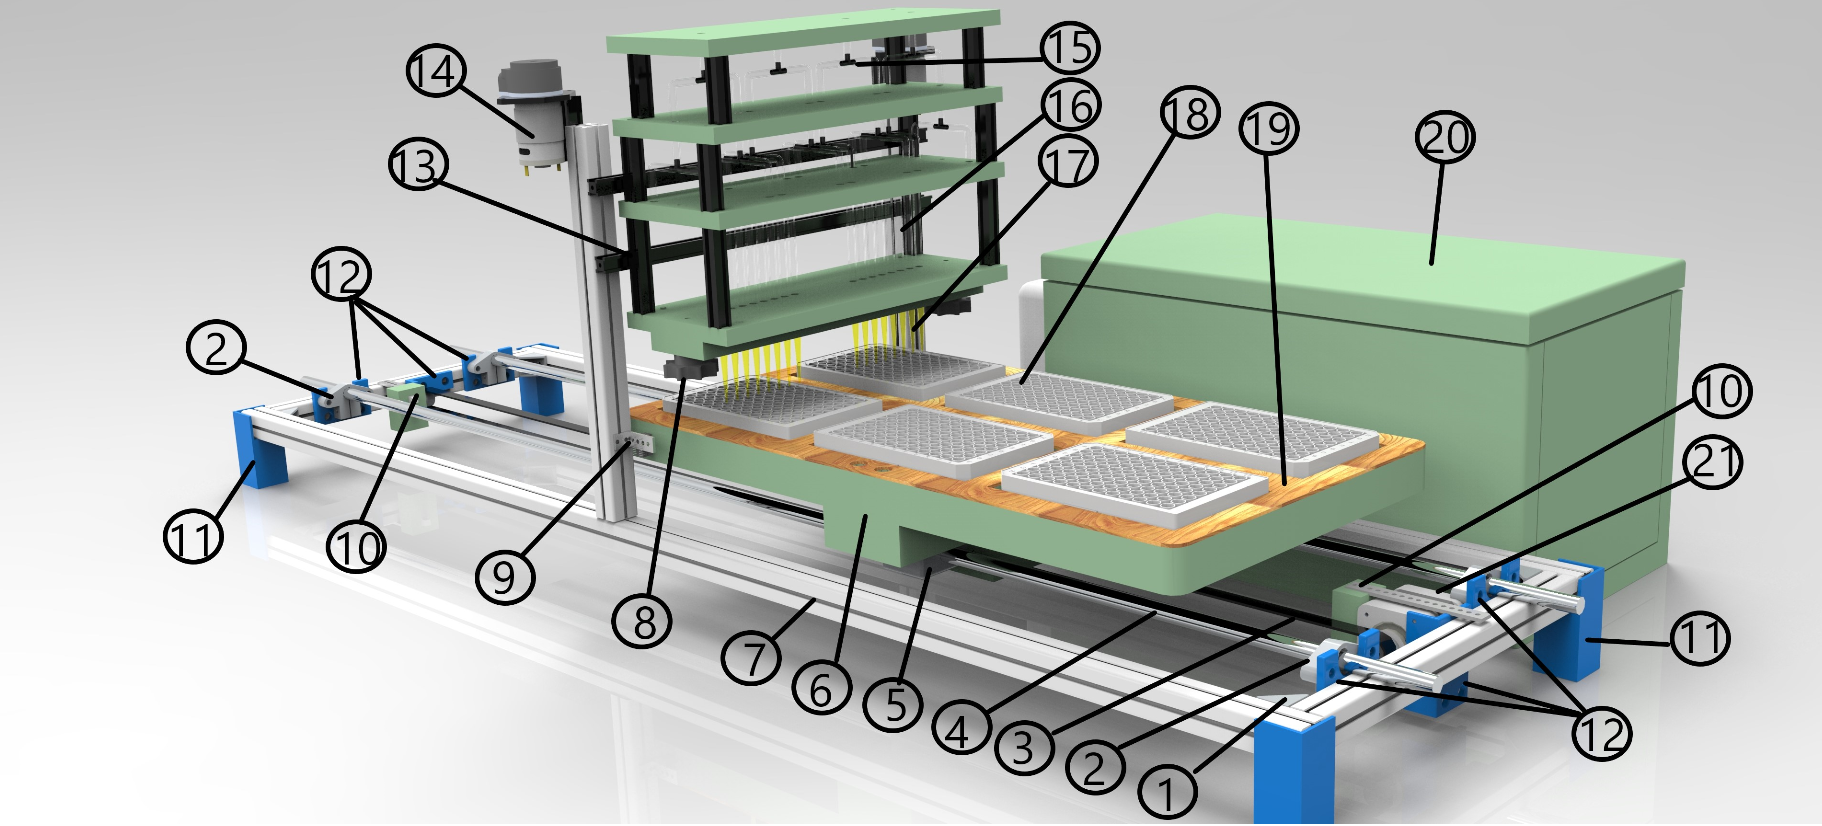
\includegraphics[width=\textwidth]{renderingBovenaanStuklijst.png}
	\caption{CAD-model bovenkant met nummer stuklijst}
	\label{fig: renderingBovenkantStuklijst}
	
\end{figure} 

\begin{figure}[h]
	\centering
	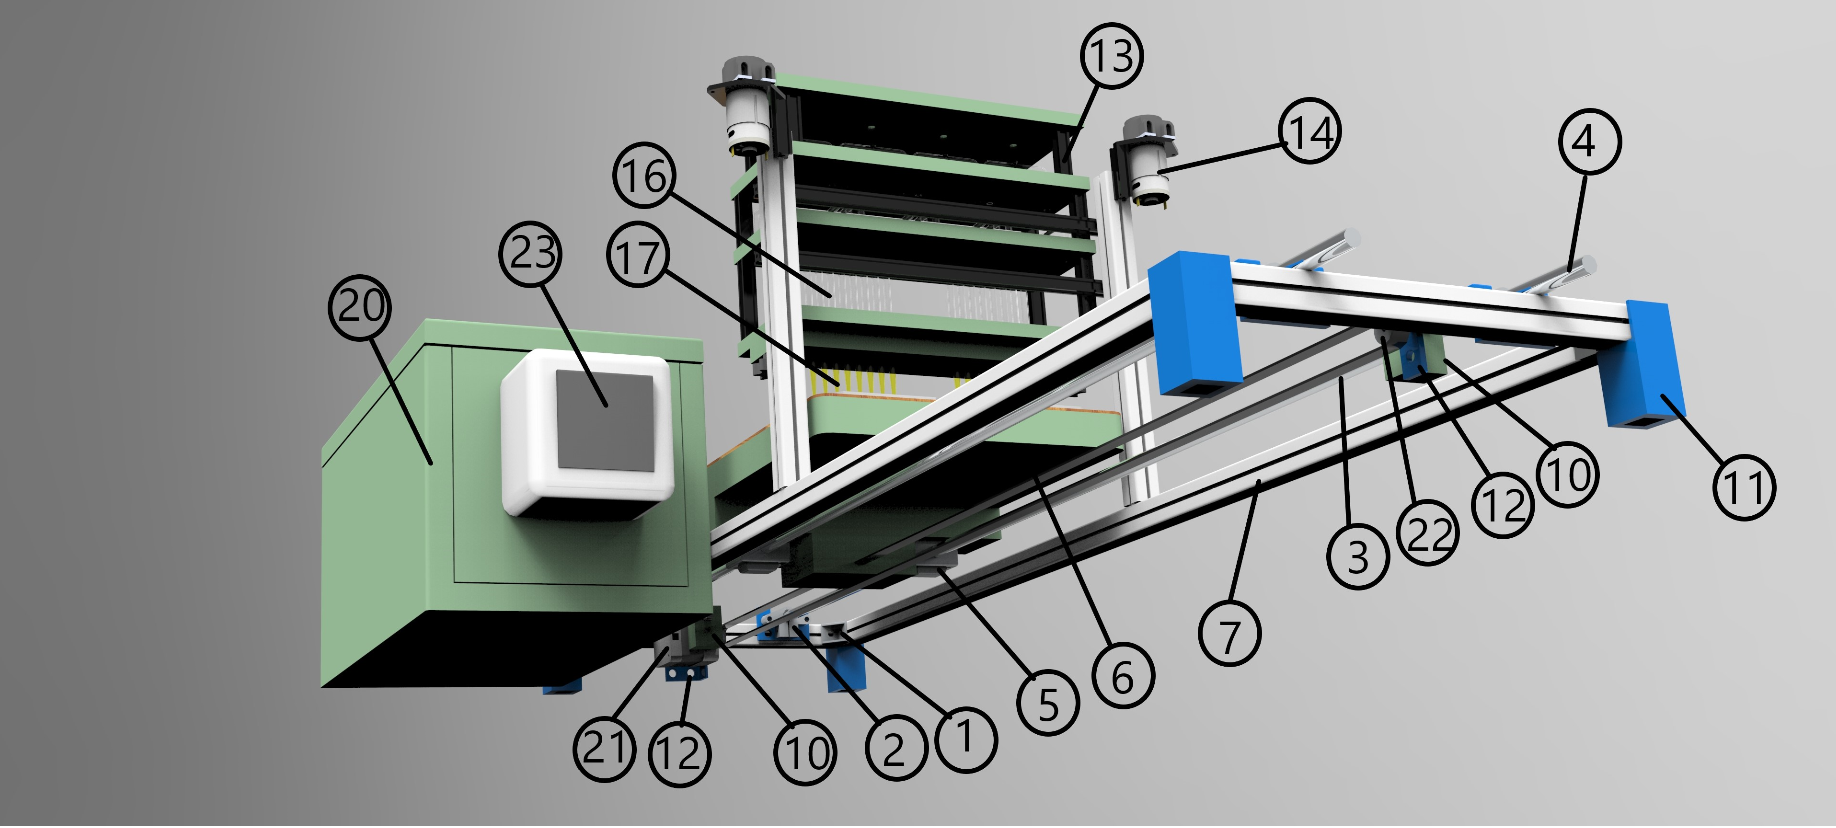
\includegraphics[width=\textwidth]{renderingOnderaanStuklijst.png}
	\caption{CAD-model onderkant met nummer stuklijst}
	\label{fig: renderingOnderkantStuklijst}
	
\end{figure} 

		

\begin{table}[!hbt]
	\noindent\makebox[\textwidth]
	\sffamily
	
	\caption{Aankopen}
		%\begin{tabular}{@{}lllll@{}}
		\begin{tabular}{|p{1cm}|p{5cm}|p{2cm}|p{2cm}|p{2cm}|}
			
		
		
		\toprule
		  Item & Product & Prijs/stuk (\euro) & Aantal & Totaal (\euro)   \\ \midrule
		1 & Aluminium hoekverbinding 2020 inclusief bevestigingsmateriaal (123-3D huismerk) & 2.75 & 4 & 11.00 \\
		2 & SHF10 as-bevestiging (2 stuks) & 9.50 & 2 & 19.00 \\
		3 & GT2 timing belt 6 mm (per meter)  & 4.50 & 2 & 9.00 \\
		4 & Staaf voor X- of Y-as glad 10 mm x 100 cm & 4.75 & 2 & 9.50 \\
		5 & SCS10UU lineaire kogellager  & 5.50 & 2 & 11.00 \\
		6 & Waterafstotend MDF \SI{2}{\metre\squared} 18 mm & 19.99 & 1 & 19.99 \\
		7 & Aluminium profiel 2020 extrusion lengte 1 m  & 9.50 & 3 & 28.50 \\
		8 & \textit{R\&D}-kosten & onbekend & &  \\
		9 & \textit{R\&D}-kosten & onbekend & &  \\
		10 & \textit{R\&D}-kosten & onbekend & & onbekend \\
		11 & \textit{R\&D}-kosten & onbekend & & onbekend\\
		12 & \textit{R\&D}-kosten & onbekend & & onbekend\\
		13 & \textit{R\&D}-kosten & onbekend & & onbekend\\
		14 & Waterpomp & onbekend & 2 & onbekend \\
		15 & Hulpstukje 4 mm Luchtslang PE T-stuk 4 x 4 x 4 mm & 0.20 & 15 & 3.00 \\
		16 & Leidingen (\si{m}) & 0.40 & 4 & 1.60 \\
		17 & Pipetpunten (zelf te voorzien) & & & \\
		18 & Microplate (zelf te voorzien) & & & \\
		19 & MDF-plaat & onbekend & & onbekend \\
		20 & Zie onderdeel 6 & & & \\
		21 & Stepper motor 42BYGHW811 NEMA-17 Bipolar 48mm & 17.95 & 1 & 17.95 \\
		22 & Spanrol | gladde pulley hoge resolutie | 6 mm riem | 5 mm as & 5.50 & 1 & 5.50 \\
		23 & Schakelaar & onbekend & 1 & onbekend \\
	    24 & GT2 Pulley hoge resolutie | 6 mm riem | 20 tanden | 5 mm as & 6.00 & 1 & 6.00 \\
	    25 & RASPBERRY PI 3 - MODELB - 1GB  & 31.59 & 1 & 31.59 \\
	    
		\bottomrule
		
		Totaal & & & & 173.63 \\
		\bottomrule
	\end{tabular}
	\label{tab:financieelVerslag}

	
\end{table}


\clearpage

\section*{Verantwoordelijkheden taakverdeling}

De volledige opdracht werd verdeeld in volgende delen (met bijhorende verantwoordelijken):
\begin{itemize}
	\item \textsc{Teamleider:} Seppe Vilain
	\item \textsc{Notulist}: Maxime Dujardin
	\item \textsc{Opstellen CAD-model}: Korneel Verkens
	\item \textsc{Mechanisme om platform met \textit{microwell}-platen te verplaatsen:} Matthias Derez, Seppe Vilain
	\item \textsc{Pompsysteem:} Maxime Dujardin, Korneel Verkens
	\item \textsc{Verslag \& presentatie:} Matthias Derez, Maxime Dujardin, Korneel Verkens, Seppe Vilain
	
\end{itemize}

\clearpage

\section*{Vakintegratie}
Om dit project tot een goed einde te kunnen brengen werden een aantal vakken uit semesters 1 t.e.m. 3 gebruikt:

\paragraph{Algemene Natuurkunde: Mechanica}

In het vak 'Mechanica' werden de basisbeginselen i.v.m. druk en stroming in dunne buizen bijgebracht. Deze kennis werd gebruikt bij het ontwerpen van het buizensysteem om de vloeistof te verdelen naar de acht microwells.

\paragraph{Beginselen van Programmeren}

De gebruikte programmeertaal voor de programma's die de machine gebruikt, is Python. In het vak 'Beginselen van Programmeren' werd deze taal geleerd. 

\paragraph{Probleemoplossen \& Ontwerpen, deel 2}

Het CAD-model werd gemaakt met het programma 'Solid Edge'. In P\&O 2 werd aangeleerd hoe hiermee te werken. Verder werd hier ook getoond hoe een Raspberry Pi microcontroller kan bestuurd worden vanaf een computer. 

\paragraph{Algemene Natuurkunde: Elektromagnetisme en Informatieoverdracht en -verwerking \& elektrische netwerken}

Deze vakken behandelen o.a. het maken en oplossen van elektrische circuits en overdracht van informatie, wat van pas kwam bij het maken van de connecties tussen de vacuümpomp, de steppermotor, de Raspberry Pi microcontroller, mosfet ... en de computer.

\clearpage

\section*{Planning}
\subsection*{Gantt-grafiek}
Op de volgende bladzijden vindt u een Gantt-grafiek van onze planning.
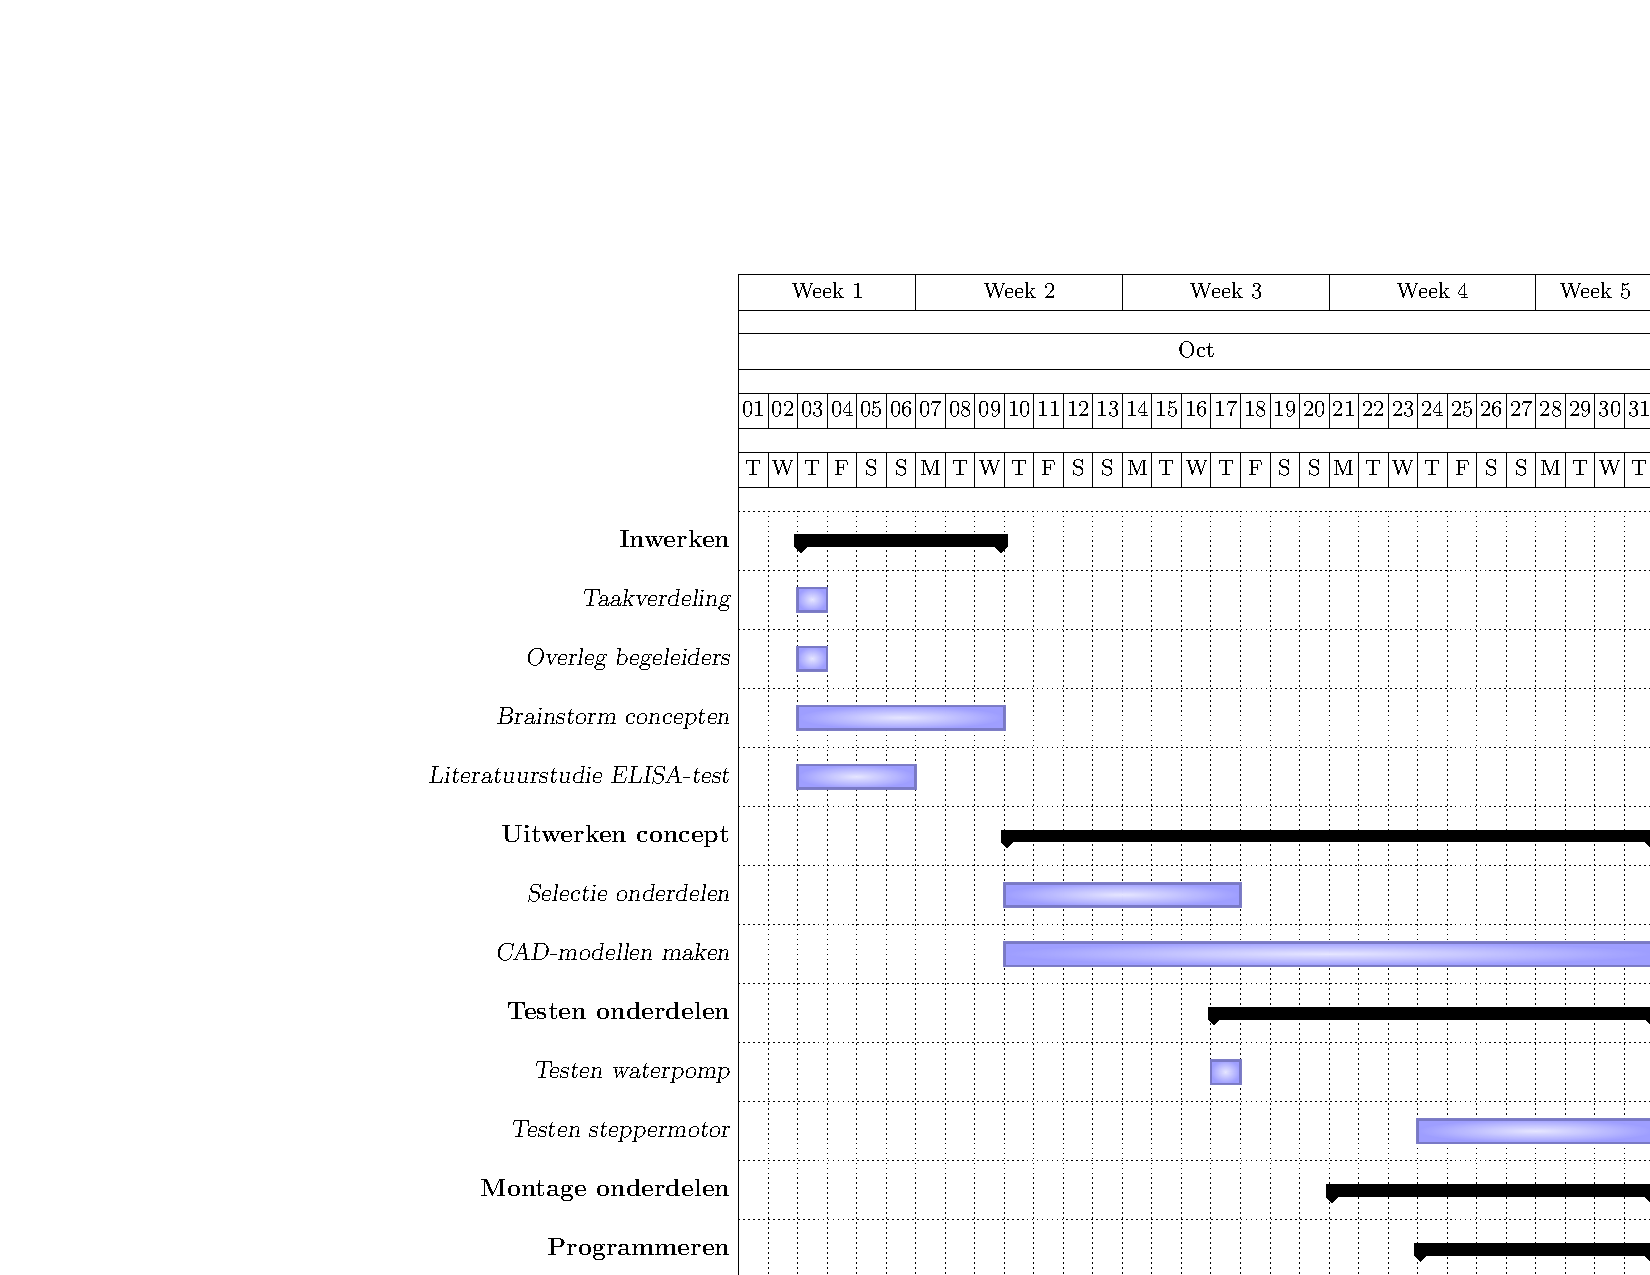
\includepdf[pages=1]{kizzigeGanttchart.pdf}
\includepdf[pages=2]{kizzigeGanttchart.pdf}
\includepdf[pages=3]{kizzigeGanttchart.pdf}







\end{document}
